\documentclass[twocolumn,twoside]{Jornadas}
\usepackage[utf8]{inputenc}
\usepackage[spanish]{babel}
\usepackage{graphicx}
\usepackage{graphics}
\usepackage{float}
\DeclareGraphicsExtensions{.eps,.ps,.pdf}
\usepackage{url}
\usepackage{lscape}
\usepackage{eurosym}

\def\BibTeX{{\rm B\kern-.05em{\sc i\kern-.025em b}\kern-.08em
    T\kern-.1667em\lower.7ex\hbox{E}\kern-.125emX}}

\newtheorem{theorem}{Teorema}


%%%%%%%%%%%%%%%%%%%%%%%%%%%%%%%%%%%%%%%%%%%%

\hyphenation{pa-ra-le-lis-mo ubi-cuos ins-ti-tu-cio-nal in-me-dia-tez ac-tua-li-dad ge-ne-ra-dos vi-sua-li-za }

\begin{document}


%\title{Sistema de información autónomo y de bajo coste para conocer el estado de las carreteras en tiempo real}
\title{Estudio de los indicadores de exposición al riesgo mediante un sistema de monitorización del tráfico basado en la tecnología Bluetooth}  
%Obtención de indicadores de exposición mediante un nuevo sistema de información de bajo coste
%Estudio de los indicadores de exposición en el área metropolitana de Granada mediante un nuevo sistema de información de bajo coste

\author{%
	P.A. Castillo, P. García-Sánchez, A.M. Mora, M.G. Arenas, \\ G. Romero, J.J. Merelo
     \thanks{Departamento de Arquitectura de Computadores. CITIC. Universidad de Granada.
	e-mail: {\tt pedro@geneura.ugr.es.}},
	P. García-Fernández
     \thanks{Departamento de Electrónica y Tecnología de Computadores. Universidad de Granada.},
	V.M. Rivas
     \thanks{Departamento de Informática. Universidad de Jaén}
}

%\author{%
%P.A. Castillo, M.G. Arenas, A.M. Mora, P. García-Sánchez, \\ G. Romero, J.J. Merelo, P. García-Fernández, V.M. Rivas
%\thanks{Departamento de Arquitectura de Computadores. CITIC. Universidad de Granada. e-mail: {\tt pedro@geneura.ugr.es.}}
%}

\maketitle
% Oculta las cabeceras y los números de página.
% Ambos elemetos se añadirán durante la edición de las actas completas.
\markboth{}{}
\pagestyle{empty} 
\thispagestyle{empty} % Oculta el número de la primera página

\begin{abstract}

%Dados los beneficios de un sistema de información sobre el estado del tráfico y del uso de la red viaria por parte de los vehículos, se plantea el desarrollo de un sistema de información de bajo coste y autónomo para monitorizar el tráfico y conocer el estado de las carreteras en tiempo real.

Los sistemas de información utilizados actualmente para la recopilación de datos y generación de información sobre el estado de las carreteras presentan dos inconvenientes: la primera es que no tienen capacidad para identificar e individualizar los vehículos que detectan. 
La segunda es su elevado coste, lo cual los hace caros para cubrir la red de carreteras secundarias. %, por lo que se suelen ubicar en vías principales y en salidas de grandes núcleos de población.

En este trabajo proponemos un sistema basado en el escaneo de los identificadores de dispositivos Bluetooth que hay en el entorno. Se trata de un identificador 
único que permite saber el fabricante e incluso distinguir de qué tipo de dispositivo se trata (PC, teléfono móvil o equipo manos libres).

%Durante el desarrollo del proyecto hemos recopilado gran cantidad de datos del paso de dispositivos bluetooth para buscar apariciones (movimientos o desplazamientos) de un dispositivo en los diferentes puntos de captación que denominaremos nodos de aquí en adelante, determinar la frecuencia de aparición de los dispositivos en un mismo nodo, calcular velocidades de movimiento entre nodos o calcular el número de dispositivos que pasan por cierto sitio cada día (ya sea festivo o laborable). 

Se ha probado el sistema en el área metropolitana de Granada, instalando seis nodos de monitorización para la recogida de datos. A partir de estos se han obtenido estadísticas con las que hemos estudiado diversos indicadores relativos al uso de vehículos por parte de la población del área monitorizada.

% Si vas a hacer énfasis en los resultados, lo que cuenta est párrafo
% debería ser el primero. ¿Qué objetivo tiene el trabajo? ¿Contar lo
% qeu se ha descubierto con ese sistema que no podría haberse
% descubierto con otro? ¿Describir el sistema? (Dado el tema de las
% jornadas, debería ser ese) 

\end{abstract}

\begin{keywords}
Ubicuidad, Tráfico, Indicadores de exposición, Sistemas de bajo coste, Monitorización, SIPEsCa
\end{keywords}


%%%%%%%%%%%%%%%%%%%%%%%%%%%%%%%%%%%%%%%%%%%%%%%%%%%%%%%%%%%%%%%
\section{Introducción}
\PARstart{D}{iversas} tareas en Seguridad Vial se basan en la obtención de indicadores de distinta naturaleza \cite{urlDGT}. Concretamente, la movilidad puede ser medida a través de distintos indicadores, conocidos con el nombre de indicadores de exposición al riesgo; los más importantes son el número de desplazamientos y los kilómetros recorridos en los mismos. 

En este trabajo presentamos un sistema de información sobre los movimientos de vehículos por la red viaria basado en la detección de dispositivos Bluetooth (BT). 

Nuestro objetivo es obtener información acerca de los flujos de tráfico que se producen en una zona, permitiendo poder gestionar de manera óptima las 
decisiones de desplazamiento por parte de los ciudadanos o desarrollar planes de actuación concretos en cada caso. 

% si el desarrollo es lo que quieres presentar, deberías concentrarte
% en eso y usarlo en el título y en el abstract. 
Para ello se ha desarrollado un dispositivo de captación autónomo y
versátil para la recogida de datos y monitorización en tiempo
real. Además se han desarrollado algoritmos de procesado de datos para
obtener estadísticas e indicadores de la exposición de los usuarios. 

El dispositivo de captación basa su funcionamiento en la detección de dispositivos BT. 
Concretamente se captarán las ondas que emiten los diferentes componentes tecnológicos que ya incorporan los vehículos, 
los accesorios que incorpora el usuario a un vehículo (GPS o kit de manos libres), así como los propios teléfonos móviles que llevan sus ocupantes.
El principal dato que se monitoriza es la dirección MAC (Media Access Control address) de la tarjeta BT de los dispositivos que son captados por el nodo. 
Se trata de un identificador único para cada dispositivo, lo que permite individualizar los vehículos que pasan.
Desde el punto de vista de la privacidad de datos, hay que destacar que los datos recopilados no se asociarán a ningún usuario ya que no existe ningún 
tipo de información que haga posible la identificación de los datos que recopilamos con una persona en concreto. 
Para ello hacemos uso de tecnologías de encriptación que imposibilitan identificar la MAC del dispositivo inalámbrico, haciendo mínima la intrusividad al hacer la recopilación de datos.


Hemos recogido una gran cantidad de datos al paso de dispositivos BT con los que hemos calculado diferentes estadísticas e indicadores sobre el uso de vehículos en la zona monitorizada, los hábitos de conducción e incluso el efecto de los factores o eventos importantes (fechas clave o tráfico en días no laborables).

La información recolectada se ha utilizado para obtener datos relativos a:
\begin{itemize}
 \item Número total de vehículos detectados por cada nodo.
 \item Número total de vehículos detectados en días laborables.
 \item Número total de vehículos detectados en días NO laborables.
 \item Número de veces que se detectan los vehículos.
 \item Tipo de recorridos que realizan los vehículos.
 \item La densidad circulatoria en diferentes horarios y diferentes tipos de vía.
 \item La velocidad media en la vía en que se dispusieron dos nodos consecutivos.
\end{itemize}

Por último, puesto que el día 14 de noviembre de 2012 fue día de huelga general en España, estudiaremos cómo afectó ésta al tráfico en el área metropolitana de Granada.


Adicionalmente se ha habilitado una web en la que se desplegará una arquitectura de servicios web \cite{Papazoglou2007,pgs2007} a través de los cuales se facilitará el acceso a la información a los usuarios.


El resto del trabajo está organizado como sigue:
En la Sección \ref{soa} se comentan las tecnologías utilizadas en la actualidad para monitorizar el tráfico que pasa por cierta zona, así como productos comerciales.
La Sección \ref{obj} detalla los objetivos planteados en este trabajo.
En la Sección \ref{hw} se presenta el dispositivo de recopilación de datos Intelify, con el que ya se ha comenzado a trabajar.
En la Sección \ref{analisis} se muestran los diferentes análisis que se han llevado a cabo a partir de los datos obtenidos.
Por último, se presentan una serie de conclusiones y trabajos futuros (Sección \ref{conclus}).


%%%%%%%%%%%%%%%%%%%%%%%%%%%%%%%%%%%%%%%%%%%%%%%%%%%%%%%%%%%%%%%
\section{Tecnologías actuales}
\label{soa}


Los sistemas de información aplicados a la recopilación de datos y generación de información sobre el estado de las carreteras 
se clasifican teniendo en cuenta la inmediatez de los datos, la exhaustividad en la recopilación y la intrusividad que tengan estos.

Los sistemas actuales, por la inmediatez de la toma de datos, pueden ser clasificados en función de la forma de su recopilación como:

\begin{itemize}
 \item De toma de datos directa: La toma de datos es directa cuando la fuente obtiene el dato estudiado sin utilizar algoritmos que, partiendo de las variables 
fundamentales del tráfico (intensidad, velocidad, ocupación o densidad), obtengan el dato de estudio calculado. Es decir cuando obtenga el dato estudiado de forma experimental.

 \item De toma de datos indirecta: en este caso el dato estudiado se obtiene a partir de la ejecución de un algoritmo, utilizando una o 
varias de las variables fundamentales del tráfico. Extrapolando, en general, los datos de un punto particular de la red a toda una sección de la misma.
\end{itemize}

Por la exhaustividad de la toma de datos, los sistemas pueden ser:

\begin{itemize}

 \item De toma de datos casi exhaustiva: Cuando su representatividad es casi total, es decir cuando el número de medidas tomadas coincida con el número de 
usuarios de ese tramo de la red.

 \item De toma de datos no exhaustiva: Cuando la fuente solo aporta datos de un número limitado de usuarios. Intentando siempre que la muestra de usuarios tenga la mayor representatividad posible.
 
\end{itemize}

Por la intrusión de la toma de datos, las tecnologías de monitorización se clasifican:

\begin{itemize}
 \item Tecnologías intrusivas: instaladas en el pavimento o a lo largo del mismo. Se basan, por tanto, en un sensor ubicado en el interior del 
paquete de firme o bien directamente sobre la calzada, es decir, en contacto con el firme (sensores de lazo inductivo, tubo neumático, 
sensores piezo-eléctricos, sensores de fibra óptica o sensores geomagnéticos). Los sensores intrusivos son, en general, más económicos 
y muy útiles para aplicaciones simples, en las que no se necesite excesiva información, aunque presentan una serie de inconvenientes: instalación y mantenimiento complejos y costosos, proporcionan información muy limitada, pueden recibir daños con facilidad, y no permiten realizar seguimientos individualizados de los vehículos.

 \item Tecnologías no intrusivas: se encuentran en posición cenital o a los lados de la carretera sin entrar en contacto con la calzada, 
causando el mínimo efecto sobre el flujo de tráfico. Para su ubicación se utilizan generalmente infraestructuras existentes. 
Son principalmente de dos tipos: activas, emitiendo una señal y captando la respuesta reflejada (radares de microondas, 
sensores ultrasónicos o los escáneres láser), o pasivas que captan variaciones producidas, en ciertos parámetros, 
por el paso de un vehículo (sensores infrarrojos, sensores acústicos o las cámaras de video). 
Por su situación, su instalación y mantenimiento puede resultar más simple que en los sensores intrusivos.

 \item Tecnologías de vehículo flotante: son aquellos sistemas en los que toda su infraestructura está contenida en un vehículo y en sistemas preexistentes (de comunicación y posicionamiento) que no afectan de forma directa a la gestión de la vía.

\end{itemize}


El sistema presentado en este trabajo se podría clasificar como de
toma de datos indirecta, no exhaustiva y no intrusiva. % ¿Esto es un
                                % resultado del trabajo? ¿Qué ventajas
                                % tiene este tipo de sistema? 


\subsection{Productos comerciales similares}

Existen diferentes empresas que trabajan en el área de la información del tráfico utilizando aproximaciones similares a la propuesta de este trabajo:

\begin{itemize}

 \item \textbf{Bit Carrier} \cite{patenteBC} \cite{BitCarrier}: Ofrece un sistema de gestión del tráfico basado en BT para realizar conteo de personas y rutas comerciales 
(pathsolver). Su tecnología se implantó en las autopistas gestionadas por Abertis para el control y monitorización del tráfico. Actualmente tiene una red de 
150 dispositivos en las autopistas de Abertis en Cataluña, lo que le permite conocer los tiempos de viaje a 200.000 personas al día.

 \item \textbf{Trafficnow} \cite{Trafficnow}: Se trata de un producto de medida del número de vehículos y tiempos de viaje basado en BT. Han implantado 
un piloto de 5 puntos de control en Vigo.

 \item \textbf{Traffax Inc} \cite{TraffaxInc}: Es una empresa que ha desarrollado productos usando BT para calcular matrices de origen-destino y tiempos de transporte entre ciudades.

 \item \textbf{Savari Networks} \cite{SavariNetworks}: Ofrece el producto comercial StreetWAVE, para monitorizar el tráfico y conocer en tiempo real el estado del tráfico.

 \item \textbf{TrafficCast} \cite{TrafficCast}: Han desarrollado modelos de predicción de movilidad en ciudades, basándose en diferentes 
combinación de tecnologías como cámaras, BT y lectura de RFIDs incluídos en los vehículos.

\end{itemize}


La propuesta presentada en este trabajo tiene algunas características
en común con las descritas anteriormente, ofreciendo funcionalidades
similares a un coste muy reducido. % ¿Una comparación de costes?
                                % ¿Todos están disponibles en España?
                                % - JJ


%%%%%%%%%%%%%%%%%%%%%%%%%%%%%%%%%%%%%%%%%%%%%%%%%%%%%%%%%%%%%%
\section{Objetivos perseguidos y resultados previsibles}
\label{obj}

%Esto debe formar parte de la introducción, aquí no opina
%absolutametne nada. - JJ
El objetivo principal es conseguir un sistema de información de bajo coste, de rápida implantación y de alta fiabilidad, tal que informe sobre las 
condiciones del tráfico en tiempo real, no sólo para las instituciones y organismos encargados de la regulación y control del tráfico, 
sino también a usuarios particulares (por ejemplo a través de alertas móviles o mediante web). 

Por tanto existen diferentes elementos en el sistema de información propuesto:

\begin{itemize}

  \item Sistema de recopilación de datos: incluye varios sensores para escanear e identificar continuamente los dispositivos BT. El sistema usa una conexión 3G para enviar los datos obtenidos al servidor de almacenamiento.
  
  \item Se han elegido localizaciones, tanto en la autovía como en ciudad, donde hay disponible alimentación a 220V.

  \item Sistema de procesado de datos para almacenar correctamente todos los datos recogidos.

  \item Servicio de información para facilitar todos los datos a los usuarios interesados en conocer el estado de las carreteras.

\end{itemize}

Así pues, se han instalado seis dispositivos para la recopilación de datos, encargados de enviar la información a los servidores para su posterior procesamiento. 
La localización de los seis nodos en el área metropolitana de Granada se detalla en la Tabla \ref{localizaciones} y se muestra con detalle en mapa de la Figura \ref{mapa}.
Dichas localizaciones se establecieron, junto con el personal de la DGT, buscando la facilidad de montaje e instalación de los dispositivos de monitorización.

 \begin{table}
 \caption{Localización de cada uno de los nodos
 \label{localizaciones}}
 \begin{center}
 \begin{tabular}{|c|l|}
 \hline
Id. Nodo  &  Localización      \\
 \hline
    1     &  C/ Julio Verne, 2    \\
 \hline
    2     &  C. Periodista Daniel Saucedo, s/n    \\
 \hline
    3     &  Plaza del Duque, s/n    \\
 \hline
    4     &  Autovía A44, km 119,550    \\
 \hline
    5     &  Autovía A44, km 123,250    \\
 \hline
    6     &  C. Goleta, 1    \\
 \hline
 \end{tabular}
 \end{center}
 \end{table}

Además, se ha configurado un
website\footnote{http://evorq.ugr.es:8080/sipesca/} con un panel de
información para conocer los principales datos de movilidad a partir
de la información recopilada en la zona monitorizada. % La página
                                % donde hay información de los nodos
                                % ya no está. - JJ


\begin{figure*}[htpb] 
\begin{center} 
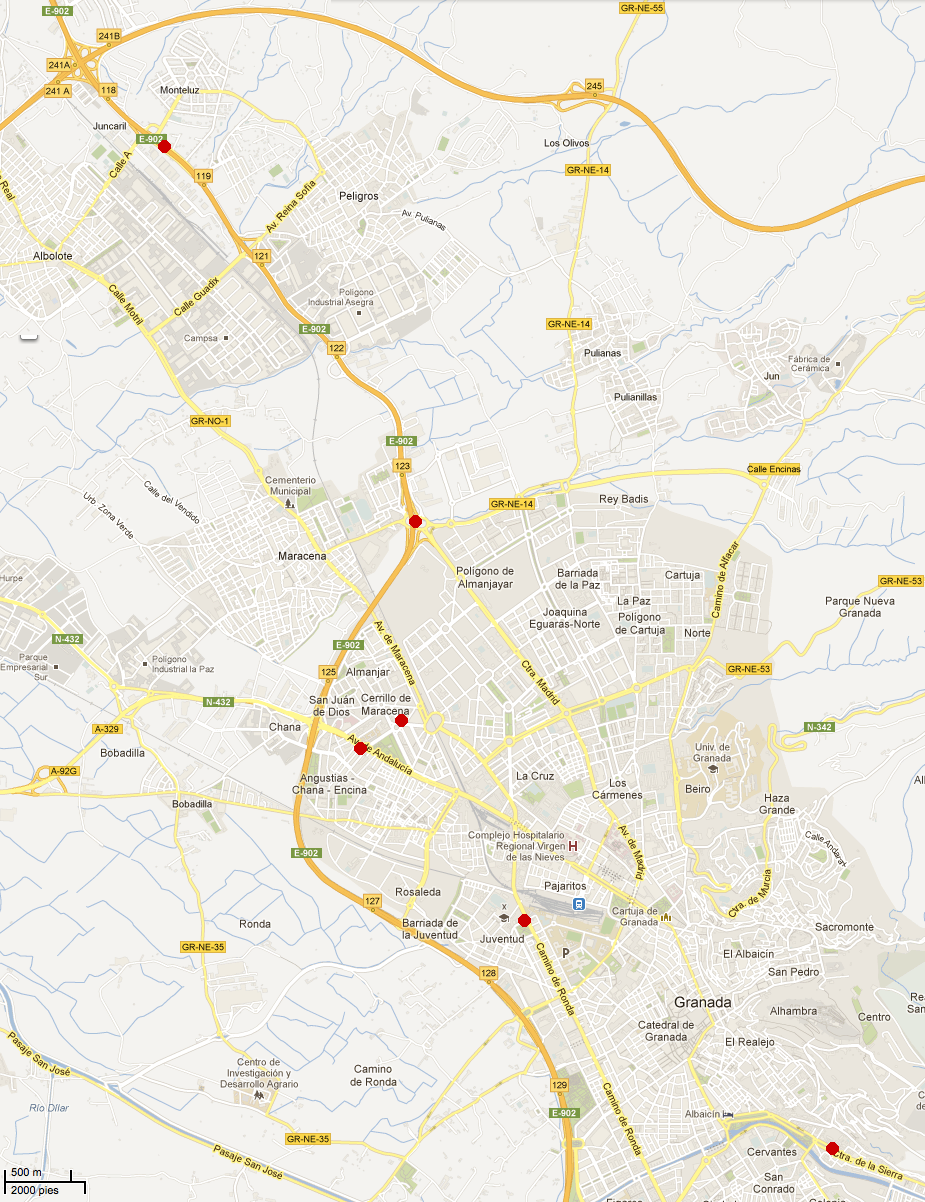
\includegraphics[scale=0.40]{mapa.png}
\end{center} 
\caption{Localización exacta en el área metropolitana de Granada de los seis nodos de monitorización} 
\label{mapa} 
\end{figure*}




%%%%%%%%%%%%%%%%%%%%%%%%%%%%%%%%%%%%%%%%%%%%%%%%%%%%%%%%%%%%%%
\section{El dispositivo hardware de recopilación de datos}
\label{hw}

Como elemento hardware para escanear los dispositivos BT presentes en un radio de acción se realizaron pruebas con un PC con Linux y una antena BT, con un dispositivo móvil con Android y con el dispositivo Intelify \cite{intelify}.

La primera opción presenta el problema del tamaño y consumo, por lo que se descartó desde un primer momento.

La segunda solución (usar dispositivos Android) presenta la ventaja de una alta autonomía y bajo consumo. Disponen de diversas opciones en cuanto a conectividad, y mediante un software sencillo pueden escanear su entorno para detectar el paso de dispositivos BT. Adicionalmente, su potencia computacional les permite realizar tareas adicionales de cómputo.

Se ha desarrollado un prototipo de aplicación\footnote{La aplicación se encuentra disponible para su descarga en la dirección http://bit.ly/16YFD8M} 
Android limitado a realizar tres tareas: observar en su entorno los dispositivos BT que pasen, almacenar los datos relativos a esos dispositivos en un archivo de texto en la memoria del teléfono, y enviar al mismo tiempo esos datos a través de la conexión 3G a un servidor que se ocupará de almacenarlos en una base de datos. 
La Figura \ref{apk} muestra la aplicación desarrollada en funcionamiento:

\begin{figure}[htpb] 
\begin{center} 
\begin{tabular}{cc}

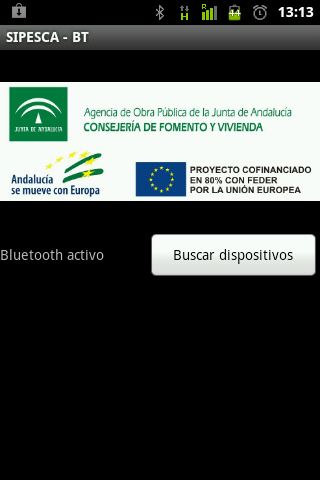
\includegraphics[scale=0.30]{CAP1.png}  &
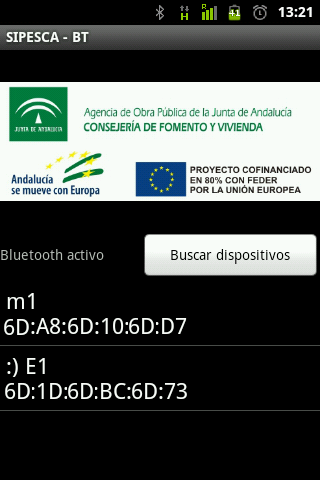
\includegraphics[scale=0.30]{CAP2.png}  \\

a & b 
 
\end{tabular}
\end{center} 
\caption{Capturas de la aplicación Android desarrollada para detectar dispositivos con el BT activado. a) muestra la aplicación lista para comenzar el escaneo; b) muestra la aplicación en funcionamiento.} 
\label{apk} 
\end{figure}

A pesar de las ventajas comentadas, esta opción presenta el problema de la baja potencia de la antena BT que montan habitualmente los móviles (para que el consumo de batería sea menor). Es más, tras comparar la capacidad de detección del móvil Android con la del PC con una antena BT externa, también se desechó esta segunda solución.


Así pues, se buscó una tercera opción cuyo consumo y tamaño fuese pequeño y al mismo tiempo tuviese una capacidad de detección alta. 
De esta forma, el desarrollo del sistema hardware se ha llevado a cabo a partir del dispositivo Intelify \cite{intelify} (ver la Figura \ref{intelify}).

\begin{figure}[htpb] 
\begin{center} 
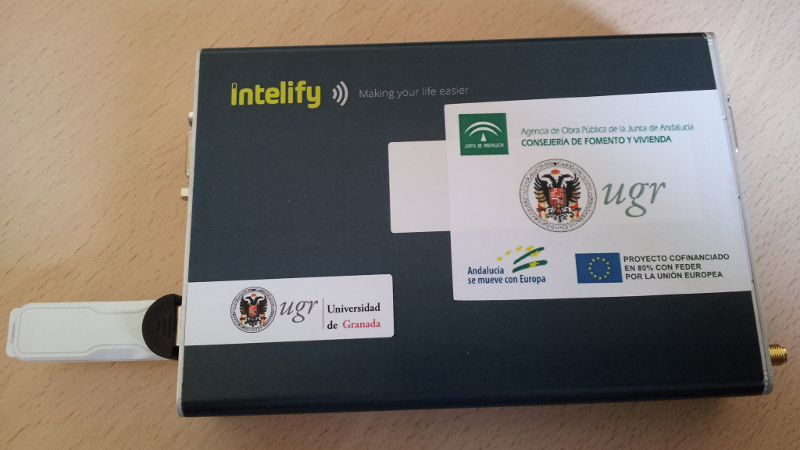
\includegraphics[scale=0.25]{intelifychisme1.png}
\end{center} 
\caption{Dispositivo Intelify con el modem USB para conexión 3G conectado.} 
\label{intelify} 
\end{figure}


El dispositivo hardware de detección está basado en la tecnología
desarrollada por Ciudad 2020 \cite{cityanalytics,Blobject} y está
compuesta básicamente por una unidad autónoma que recopila información
del entorno, siendo capaz de enviar la información a unos servidores
centrales que interpretan la información.  %Esto no lo has anticipado
                                %en la intro. Si has hecho esto y es
                                %un resultado la evaluación de los
                                %diferentes dispositivos, di en la
                                %introducción  que es uno de los
                                %objetivos. 
La Tabla \ref{caracteristicas} detalla las características principales del dispositivo.


\begin{table*}[htpb]
\caption{Características técnicas del dispositivo Intelify utilizado como hardware de monitorización.}
\label{caracteristicas}
\begin{center}
 {\footnotesize
\begin{tabular}{|c|c|}
\hline
Dimensiones & 113 x 163 x 30 mm. \\
\hline
     & Encendido  \\
LEDs & Red 3G activa  \\
     & Red Ethernet activa  \\
\hline
				& Ethernet  \\
Comunicaciones	& Antena WiFi  \\
				& Antena Bluetooth  \\  
				& Modem 3G USB  \\
\hline
Puertos USB & Un puerto USB para la antena City Analytics   \\
			& Un puerto USB para conexión 3G  \\
\hline
Otros puertos & Conector RS-232   \\
			  & Contector VGA  \\
\hline
 			 & 18 V - 1200mA    \\
Alimentación & Conector jack estándar 5,5 mm. \\
			 & exterior y 2,1 mm. interior  \\
\hline
Comunicación & Conector RJ45 para red Ethernet   \\
			 & Modem USB para conexión 3G  \\
\hline
Antenas & Antena USB City Analytics   \\
		& Antena WiFi  \\
\hline
Micrófono & Sensor de ruido  \\
\hline
Sensor de temperatura & Sensor de temperatura en placa con extrapolación  \\
\hline
Cajas   & Caja de aluminio de 1,5 mm   \\
		& Posibilidad de exterior  \\
\hline
Sistema operativo & Debian 6.0 	Squeeze  \\
\hline
\end{tabular}
 }
\end{center}
\end{table*}


Este dispositivo cuenta con una serie de sensores que permiten interpretar la información del entorno, entre otras, el flujo de personas/vehículos que pasan.

%La tecnología desarrollada por Ciudad 2020 y los servicios que ofrece se basan en la implantación de una red de dispositivos Intelify para captar información del entorno físico y ayudar en la toma de decisiones a todo tipo de organizaciones en función del análisis del flujo y comportamiento de las personas.

%Mediante un despliegue de dispositivos autónomos por la ciudad, estos dispositivos ofrecen información de importancia para los sectores turístico y comercial, entre otros, así como para la movilidad en la ciudad. Concretamente, en \cite{numerodepersonas} se ofrece un servicio de monitorización del paso de personas por las calles céntricas de la ciudad de Córdoba.

% El coste de esta solución es de 1000 euros por dispositivo, incluyendo costes de mantenimiento informático de forma remota, comunicación mediante telefonía 3G y almacenamiento y gestión de los datos. 

Frente a otras tecnologías, la representatividad de los datos es bastante precisa, estimándose a priori un $8,5\%$ de error en las detecciones, tal y como demuestra el estudio aproximativo al error medio \cite{estudioprecision}.


%%%%%%%%%%%%%%%%%%%%%%%%%%%%%%%%%%%%%%%%%%%%%%%%%%%%%%%%%%%%%%
\section{Obtención y análisis de los datos obtenidos}
\label{analisis}

A continuación se muestra el análisis de los datos recopilados durante el periodo de monitorización (del 8 de noviembre al 9 de diciembre, ambos inclusive) para obtener estadísticas 
para el estudio del comportamiento de los vehículos en la zona
monitorizada. % Di qué licencia tienen los datos y qué hay que citar
              % si se usan. 

Concretamente, en las siguientes subsecciones, se ofrece información acerca del número total de vehículos detectados por cada nodo, en días laborables o festivos, sobre la densidad del tráfico por rango horario, acerca de los desplazamientos individuales, y de la velocidad media en un tramo delimitado por dos nodos consecutivos.

Por último, puesto que el día 14 de noviembre de 2012 se celebró una huelga general, estudiaremos cómo afectó la huelga al tráfico en el área metropolitana de Granada, comparando los totales de detección de dispositivos entre el día de la huelga (14 de noviembre), y el día siguiente (15 de noviembre).



\subsection{Total de vehículos detectados (laborables y festivos)}
 % VehiculosTotales.txt tiene los vehículos totales detectados en cada nodo.

En la primera parte del análisis se muestran el número de dispositivos detectados por cada uno de los nodos instalados.

 \begin{table}
 \caption{Número de dispositivos BT totales detectados en cada uno de los nodos.
 \label{VehiculosTotales}}
 \begin{center}
 \begin{tabular}{|c|c|}
 \hline
Id. Nodo  &  N. de dispositivos detectados  \\
 \hline
    1     &    31408  \\
 \hline
    2     &    45032  \\
 \hline
    3     &    33165  \\
 \hline
    4     &    358494  \\
 \hline
    5     &    297874  \\
 \hline
    6     &    7872  \\
 \hline
 \end{tabular}
 \end{center}
 \end{table}

En total se han detectado 773845 dispositivos BT por alguno de los seis nodos. 
Como se observa en la Tabla \ref{VehiculosTotales}, los dos nodos situados en la autovía de Sierra Nevada 
(A44, Circunvalación de Granada, nodos 4 y 5) son los que más datos han recopilado, mientras que el situado en una calle 
secundaria (nodo 6) ha sido el que menos.



\subsection{Total de vehículos detectados en días no laborables}
 % VehiculosFestivos.txt tiene los vehículos detectados en día festivo en cada nodo.

A continuación, y para comparar la intensidad circulatoria entre días laborables y no laborables, se ha calculado el número de pasos en días festivos y no laborables.

 \begin{table}
 \caption{Número de dispositivos BT totales detectados en cada uno de los nodos exclusivamente en días no laborables.
 \label{VehiculosFestivos}}
 \begin{center}
 \begin{tabular}{|c|c|}
 \hline
Id. Nodo  &  N. de dispositivos detectados  \\
 \hline
    1     &    2149  \\
 \hline
    2     &    2804  \\
 \hline
    3     &    2832  \\
 \hline
    4     &    32182  \\
 \hline
    5     &    24166  \\
 \hline
    6     &    1269  \\
 \hline
 \end{tabular}
 \end{center}
 \end{table}

La Tabla \ref{VehiculosFestivos} muestra un descenso en el número de dispositivos detectados por todos los nodos en días no laborables, frente al número de 
detecciones en días laborables. Aún así, los nodos situados en la autovía de Sierra Nevada siguen recogiendo muchos más datos que el resto, debido al 
tráfico denso que soporta esta vía en días no laborables, puesto que son puntos de paso para ir a zonas comerciales o de entrada y de salida del núcleo urbano de Granada hacia otros
núcleos como Jaén, Murcia, Madrid, etc.



\subsection{Densidad del tráfico en la vía por horas}
 % VehiculosDiferentesPorHoras.txt contiene para cada uno de los nodos, los dispositivos diferentes detectados en cada rango horario (final de la línea)

La densidad circulatoria por horas podemos calcularla a partir del total de dispositivos diferentes detectados en cada rango horario en cada nodo. Es decir, 
hemos tenido en cuenta sólo los dispositivos BT que han pasado por cada nodo, según el rango horario, pero sin tener en cuenta pasos repetidos del mismo dispositivo por el mismo nodo.
Esta medición incluye dispositivos, no pasos de estos dispositivos.

 \begin{figure}[htb]
 \begin{center}
 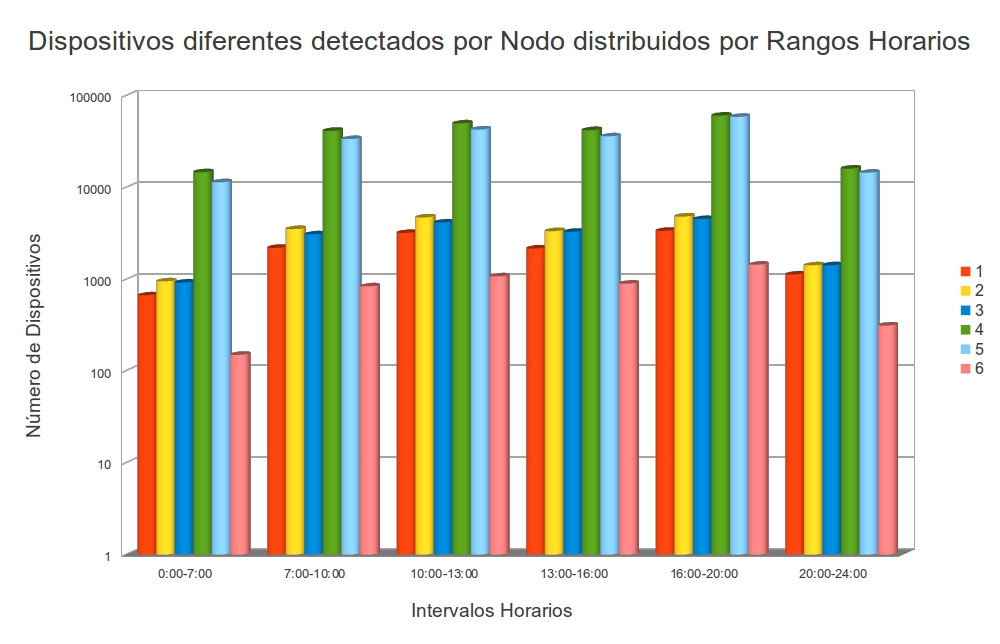
\includegraphics[scale=0.20]{VehiculosDiferentesPorHoras.jpg}
 \caption{Para cada uno de los nodos se muestra el total de dispositivos diferentes detectados en cada rango horario. Para cada rango de horas se muestra el total detectado en cada uno de los seis nodos. La figura se muestra en escala logarítmica.
 \label{VehiculosDiferentesPorHoras}}
 \end{center}
 \end{figure}
 % Gráfica (histograma) de la densidad de la vía por horas: desde las 00-7h, de 7-10h, de 10-13h, de 13-16h, de 16-20h, y de 20-24h.
 
La Figura \ref{VehiculosDiferentesPorHoras} muestra mayor densidad, en todos los nodos, durante las denominadas horas punta de entrada o salida para ir al trabajo y/o colegios.



\subsection{Detecciones totales por rango horario}
 % VehiculosPorHoras.txt indica para cada nodo, el número de dispositivos detectados en el rango horario, sin diferenciar si el dispositivo es siempre el mismo o no. 


Adicionalmente podemos calcular para cada nodo, el número de pasos totales de los dispositivos en cada rango horario, incluyendo repeticiones del mismo dispositivo. 
Así pues, se incluirán pasos repetidos del mismo vehículo.

 \begin{figure}[htb]
 \begin{center}
 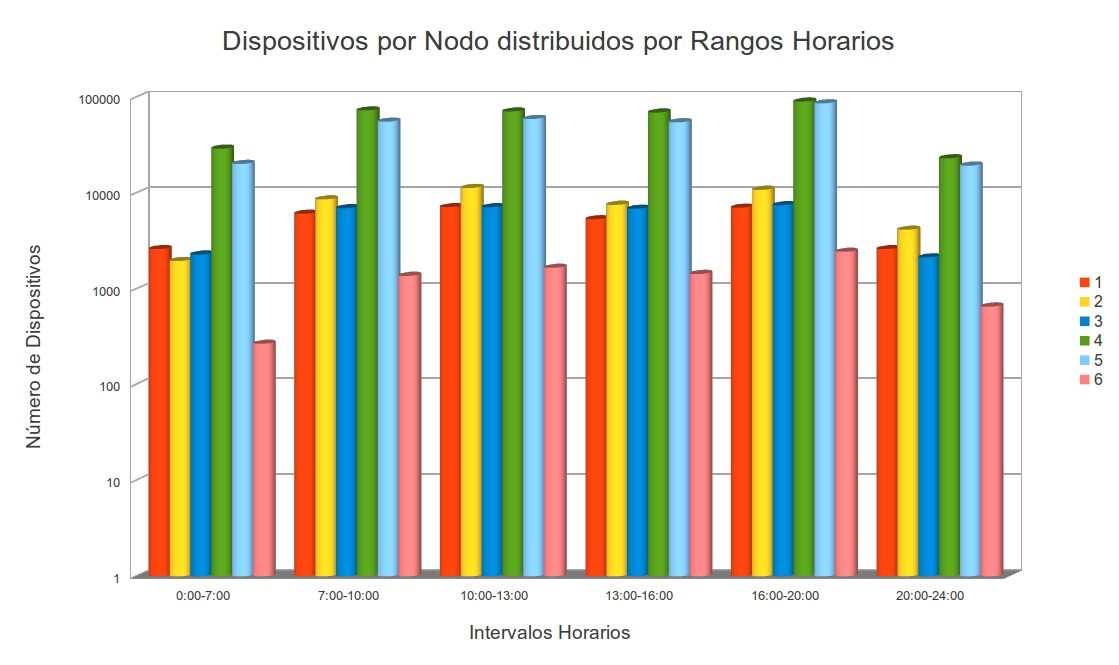
\includegraphics[scale=0.20]{VehiculosPorHoras.jpg}
 \caption{Para cada uno de los nodos se muestra el total de pasos detectados en cada rango horario. Para cada rango de horas se muestra el total detectado en cada uno de los seis nodos. La figura se muestra en escala logarítmica.
 \label{VehiculosPorHoras}}
 \end{center}
 \end{figure}
 
Al igual que en el caso anterior, en la Figura \ref{VehiculosPorHoras} observamos una mayor densidad circulatoria en todos los nodos, en horas punta de entrada o salida del trabajo y colegios.



\subsection{Número de apariciones de los vehículos individualizados}
 % Intervalos.txt contine el número de vehículos detectados entre 0 y 5 veces, entre 5 y 10 veces y así sucesivamente hasta más de 25 veces detallado en cada nodo.

A continuación podemos sacar partido de la capacidad del sistema propuesto para individualizar los dispositivos BT, pudiendo detectar si esos mismos 
vehículos repiten paso por diferentes nodos.

 \begin{figure}[htb]
 \begin{center}
 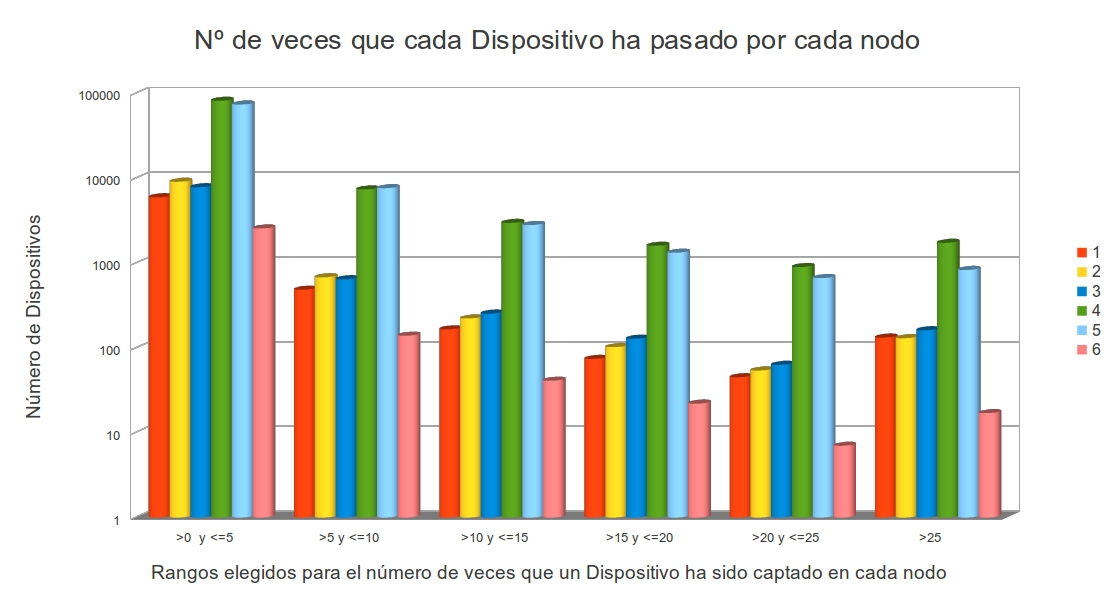
\includegraphics[scale=0.20]{Intervalos.jpg}
 \caption{Para cada uno de los nodos se muestra el total de dispositivos detectados cierto número de veces (repetidas apariciones del mismo dispositivo). La figura se muestra en escala logarítmica.
 \label{Intervalos}}
 \end{center}
 \end{figure}
 
 % Histograma que muestre cuántos coches se detectan entre una y 5 veces, entre 6 y 10, entre 10 y 20, y más de 20 veces.

En la Figura \ref{Intervalos} podemos ver que hay una gran cantidad de vehículos que repiten su paso por ciertos nodos (principalmente los situados en la A44) hasta 10 veces. 
Incluso se puede ver que en los nodos 4 y 5 hay alrededor de 1000 vehículos que repiten su paso más de 25 veces. En el resto de nodos, más de 25 repeticiones del mismo dispositivo 
se han detectado alrededor de 120 veces solamente.



\subsection{Complejidad de los desplazamientos}
 % NodosPorDondePasan.txt contiene el número de vehículos que han pasado por 2 nodos, por 3 nodos y así hasta por los 6 nodos y el número medio de veces que han pasado 2, 3, 4, 5 o 6 veces por cada nodo.

En el estudio de la complejidad de los desplazamientos se han calculado el número de vehículos que han pasado por 2 nodos, por 3 nodos y hasta 6 nodos. 
En la Tabla \ref{tNodosPorDondePasan} se muestra además el número medio de veces que han pasado los vehículos por 2, 3, 4, 5 o 6 nodos

 \begin{table*}[hptb]
 \caption{Número de vehículos que han pasado por 2 nodos, por 3 nodos
   y hasta 6 nodos, y el número medio de veces que han pasado los
   vehículos por 2, 3, 4, 5 o 6 nodos. En algunos casos las
   desviaciones son altas debido a que algunos dispositivos tienen un
   número muy alto de apariciones en algunos de los nodos. % Deberías
                                % poner no la desviació estándar, sino
                                % el error de la media. Tampoco queda
                                % claro la media de qué es... - JJ \label{tNodosPorDondePasan}}
 \begin{center}
 \begin{tabular}{|c|c|c|c|}
 \hline
 Núm. nodos & 	Núm. dispositivos & 	Total de pasos & 	Media $\pm$ Desv. Estándar  \\
 \hline
1 & 	72989 & 	 165033 & 	$2.26 \pm 31.16$  \\
 \hline
2 & 	53947 & 	 425667 & 	$7.89 \pm 11.48$  \\
 \hline
3 & 	8125 & 	 131570 & 	$16.19 \pm 24.71$  \\
 \hline
4 & 	1359 & 	 39241 & 	$28.88 \pm 140.82$  \\
 \hline
5 & 	254 & 	 8603 & 	$33.87 \pm 59.51$  \\
 \hline
6 & 	61 & 	 3731 & 	$61.16 \pm 94.78$  \\
 \hline
 \end{tabular}
 \end{center}
 \end{table*}

La información anterior se complementa visualmente con la Figura \ref{fNodosPorDondePasan}, en la que se muestra (en escala logarítmica) cuántos coches pasan sólo 
por un nodo, por dos nodos, por tres nodos, etc. En este caso el eje de la variable independiente (X) representa el número de veces que han sido detectados y no el número de nodo (id) en el que se ha 
recolectado el dato.

 \begin{figure}[htb]
 \begin{center}
 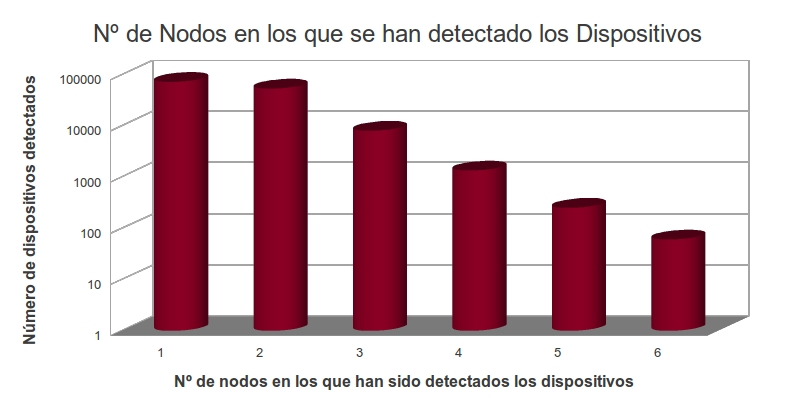
\includegraphics[scale=0.20]{NodosPorDondePasan.jpg}
 \caption{La figura muestra cuántos coches pasan sólo por un nodo, por dos nodos, por tres nodos, etc. Para mejorar la visualización, en esta gráfica se ha utilizado escala logarítmica.
 \label{fNodosPorDondePasan}}
 \end{center}
 \end{figure}
 % Histograma que muestre cuántos coches pasan sólo por un nodo, por dos nodos, por tres nodos, etc.

Como se esperaba, gran parte de los dispositivos BT pasan pocas veces por casi todos los nodos, mientras que la mayoría pasa sólo por uno o dos de ellos 
(sus desplazamientos se centran en una parte de la zona monitorizada).


 
\subsection{Efecto de la huelga del 14-N al tráfico de la zona}

Justo en mitad del periodo de monitorización, en España se celebró un día de huelga general (14 de noviembre de 2012), lo que ha quedado reflejado en la cantidad de coches detectados en los diferentes nodos.

Se ha analizado el efecto de la huelga general en el tráfico de la zona monitorizada, mostrando en la Tabla \ref{huelga} el número de pasos detectados el día 14 de noviembre y justo el día siguiente.

%Deberíais compararlo con el día 7 y el 21 y con la media de ambos en
%vez de con el día anterior o el siguiente. Cada día tiene un tráfico
%característico - JJ 
 \begin{table}
 \caption{Comparación del número de pasos por cada nodo entre el día de la huelga general (14 de noviembre) y el día siguiente. No aparece recogido el nodo 1 debido a que el dispositivo hardware sufrió un problema de alimentación durante un par de días en esas fechas.
 \label{huelga}}
 \begin{center}
 \begin{tabular}{|c|c|c|}
 \hline
 Nodo  &  Total de pasos  & Total de pasos  \\
       &  (14-nov) & (15-nov) \\
 \hline
 2	& 1841  & 2722  \\
 \hline
 3	& 891   & 1169 \\
 \hline
 4	& 10807	& 16942 \\
 \hline
 5	& 831  	& 4017\\
 \hline
 6	& 946   & 1419 \\
 \hline
 \end{tabular}
 \end{center}
 \end{table}

En la Tabla \ref{huelga} se aprecia un número de vehículos detectados menor el día de la huelga respecto al día siguiente (día laborable en el que la actividad fue normal en la zona).



\subsection{Análisis de la velocidad de los vehículos entre dos nodos consecutivos}
 % tabla de la velocidad media de los vehículos en el tramo (en laborables y en fin de semana).
 % El "Granada 5" está en el km 123,250 ; el "Granada 4" está en el km 119,550 ; hay 3700 metros entre ambos. 

Por último, a partir de los dos nodos consecutivos localizados en la autovía A44, podemos calcular velocidades medias en el tramo delimitado por los nodos 4 (situado en el km 119,550) 
y 5 (situado en el km 123,250) de un total de 3700 metros. 
En realidad podemos calcular la velocidad media en el tramo a nivel global, no la velocidad a la que ha ido cada vehículo en cada instante dentro del tramo.

 \begin{table}
 \caption{Velocidades medias (a nivel global) en el tramo delimitado por los nodos 4 y 5 situados en la autovía de Sierra Nevada.
 \label{velocidad}}
 \begin{center}
 \begin{tabular}{|c|c|}
 \hline
Rango de velocidad (km/h) &  Número de pasos  \\
 \hline
v$\leq$60.0	& 1495  \\
 \hline
60.0$\leq$v$\leq$70.0 & 2585  \\
 \hline
70.0$\leq$v$\leq$80.0 & 7421  \\
 \hline
80.0$\leq$v$\leq$90.0 & 16339  \\
 \hline
90.0$\leq$v$\leq$100.0 & 20144  \\
 \hline
100.0$\leq$v$\leq$120.0 & 14384  \\
 \hline
120.0$\leq$v$\leq$140.0 & 5434  \\
 \hline
v$\geq$140.0 & 1326  \\
 \hline
 \end{tabular}
 \end{center}
 \end{table}


En dicho tramo, la velocidad está limitada a 100 km/h. Sin embargo, y aunque la gran mayoría respetan el límite, vemos que una gran cantidad de coches superan dicha limitación.



%%%%%%%%%%%%%%%%%%%%%%%%%%%%%%%%%%%%%%%%%%%%%%%%%%%%%%%%%%%%%%
\section{Conclusiones y Trabajos Futuros}
\label{conclus}

 % Estudio de los indicadores de exposición en el área metropolitana de Granada mediante un nuevo sistema de información de bajo coste
 % Obtención de indicadores de exposición mediante un nuevo sistema de información de bajo coste

Los sistemas de información utilizados actualmente para la recopilación de datos sobre el estado de las carreteras carecen de la capacidad para individualizar los vehículos que detectan, o bien presentan un elevado coste.

En este trabajo se ha presentado un nuevo sistema de información de bajo coste para monitorizar el tráfico en diferentes tipos de vías en tiempo real.

El objetivo principal ha sido en todo momento la obtención de indicadores de exposición mediante un nuevo sistema basado en la detección de dispositivos BT que pasan por diferentes nodos de información.
De esta forma, hemos podido monitorizar la densidad de tráfico y los desplazamientos realizados por los usuarios, individualizando los vehículos conforme se mueven entre nodos dentro de la zona.

Así pues, se han estudiado diferentes soluciones para desarrollar un dispositivo hardware de detección, habiendo descartado algunas por costosas, por su alto consumo o por su corto alcance en el escaneo.

Además, se han tenido en cuenta diferentes tipos de vía, con muy distintos tipo de tráfico. 
También se han obtenido estadísticas en función de los días de la semana y de los horarios de circulación.


Se han realizado diversos análisis de los datos recopilados durante el periodo de monitorización (del 8 de noviembre al 9 de diciembre de 2012) para obtener diferentes estadísticas.

Concretamente, se ha estudiado el número total de vehículos detectados por cada nodo, en días laborables o festivos. También se ha estudiado la densidad del tráfico por rango horario, y los desplazamientos individuales.

Por último, se ha analizado la velocidad media en un tramo delimitado por dos nodos consecutivos.


Finalmente, ha quedado demostrada la potencia y funcionalidad del sistema, que se complementa con el desarrollo de un conjunto de servicios web para facilitar el acceso a la información en tiempo real, pudiendo realizar diferentes tipos de consultas.


Como trabajos futuros se abren diversas líneas de investigación, centradas principalmente en el procesamiento de los datos recogidos mediante algoritmos complejos de minería de datos \cite{Trevor2009}, computación evolutiva \cite{Eiben2003,Michalewicz2004,Yang2010} y redes neuronales \cite{Castillo2001,Rivas2003,Castillo2007}, aprendizaje automático \cite{Arenas2005} y de métodos estadísticos \cite{Jiawei2006,Hill2007,Nisbet2009}, que se irán desarrollando e integrando como servicios web \cite{Papazoglou2007,pgs2007} en el sistema.
La idea es desarrollar en el futuro un sistema de predicción y ayuda a la toma de decisiones, capaz de aplicar conocimiento en aplicaciones relacionadas con la movilidad. 


Se espera que el desarrollo e implantación de este tipo de sistemas ofrezca una serie de servicios de información con valor añadido que no se consiguen con las tecnologías actuales.


\bigskip

%%%%%%%%%%%%%%%%%%%%%%%%%%%%% AGRADEC. %%%%%%%%%%%%%%%%%%%%%%%%%%%%%%%%%%%
\section*{Agradecimientos}

\begin{figure}[H]
\begin{center} 
 
\includegraphics[scale=0.7]{logos_SIPESCA_2.jpg}
\end{center} 
%\caption{ } 
%\label{logos_SIPESCA_2} 
\end{figure}

Este trabajo se está desarrollando gracias a la financiación del proyecto FEDER de la Unión Europea con título
{''Sistema de Información y Predicción de bajo coste y autónomo para conocer el Estado de las Carreteras en tiempo real mediante dispositivos distribuidos'' (SIPEsCa)}
del Programa Operativo FEDER de Andalucía 2007-2013. 
Asimismo, queremos mostrar nuestro agradecimiento al personal e investigadores de la Agencia de Obra Pública de la Junta de Andalucía, Consejería de Fomento y Vivienda, por su dedicación y profesionalidad.


\bigskip


%{SIPEsCa} (G-GI3000/IDIF) de la Consejería de Obras Públicas y Vivienda de la Junta de Andalucía,

%The authors would like to thank the FEDER of European Union for financial support via project 
%{''Sistema de Información y Predicción de bajo coste y autónomo para conocer el Estado de las Carreteras en tiempo real mediante dispositivos distribuidos'' (SIPEsCa)}
%of the Programa Operativo FEDER de Andalucía 2007-2013. We also thank all Agency of Public Works of Andalusia Regional Government staff and researchers for their dedication and professionalism.


%The authors are grateful to anonymous referees for their constructive comments and advice about the first version of our paper.
%The authors are very grateful to the anonymous referees whose comments and suggestions have contributed to improve this paper.

\nocite{*}

\bibliographystyle{Jornadas}

\bibliography{referencias} 

\end{document}

